\chapter{Introduction}

\drop{E}{arth} Observation (\acs{EO}) commercial data sales have increased a 550\% in
the last decade~\cite{Euroconsult2010}. This area is considered a key element in the
space industry and an opportunity market for the next years.

\ac{EO} industries implement on-premises conventional infrastructures to acquire,
store, process and distribute the geo-information generated.

However these solutions have the risks of over/under size the infrastructure, they are not flexible to cover sudden changes in the demand of services and the access to the information presents large latencies.  These aspects limit the use of \ac{EO} technology for real time use such as to manage crises, natural disasters and civil security among others~\cite{Deren2007}.

In addition, new sectors and user typologies are applying for new \ac{EO} services
and there is an increasing demand of this services. These users
need more flexible, easy and instant access to \ac{EO} products and services through
the Web. This demand has traditionally been driven through Space Data
Infrastructures and heavy standards (\acs{ISO} TC/211 and \ac{OGC}) which are focused on
interoperability rather than the real demand from the end-users.

The use of cloud computing technology can overcome the previously defined limitations that present conventional infrastructures because of its elasticity, scalability and on-demand use characteristics~\cite{Ambrust2010}.

The GEO-Cloud experiment goes beyond conventional data infrastructures used in
the \ac{EO}
industry and beyond the implementations of applications running in cloud, to
quest which parts of a complete infrastructure of \ac{EO} are technologically and
economically viable to be virtualized to offer basic and high added value
services (see Figure~\ref{fig:intr-geocloudConcept}).

\begin{figure}[!h]
\begin{center}
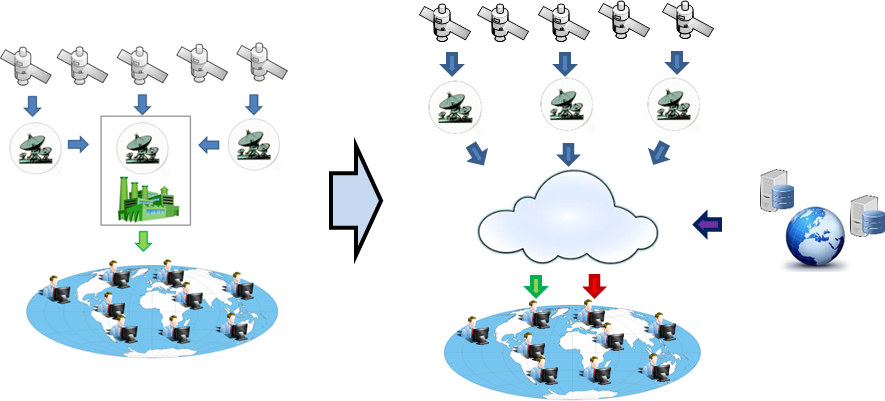
\includegraphics[width=0.9\textwidth]{statement/geocloudConcept.png}
\caption[The GEO-Cloud Concept.]{The GEO-Cloud Concept. It is based on the use of cloud technology to acquire data, store it, process it, integrate it with other sources and distribute it to end users with the final objective of testing viable solutions for its real implementation.}
\label{fig:intr-geocloudConcept}
\end{center}
\end{figure}

The GEO-Cloud experiment is is divided into two sub-experiments~\cite{PEREZ}:
\begin{itemize}
\item One experiment in a system integrated in \vw and \bonfire cloud emulating
  the whole \ac{EO} system. In \vw, the constellation of satellites and the
  ground stations are simulated. In the \bonfire cloud, the novel architecture
  for \ac{EO} images processing is implemented. Both \vw and \bonfire are
  interconnected for simulating the data transfers between the satellites and
  ground stations and between the ground stations and the cloud platform.
\item One experiment based in \pl. The experiment consists of real networks
  interconnected around the world, which are used to emulate the real behaviour
  of the links between the ground stations and the cloud and from the cloud to
  the end users. The network bandwidth, loss-rate and delay were measured. Those
  parameters, once measured were used to update the parameters of the network
  models implemented in \vw.
\end{itemize}

GEO-Cloud  emulates the remote sensing mission with emulated satellites, the
topology network and the communications in the \vw testbed. The data
acquired from the emulated satellites is transferred to the \bonfire cloud
for storage, processing and distribution to end users. End users accessing and
broadcasting will be emulated in another network implemented in \vw. In
order to implement realistic impairments in \vw, real networks will be
tested in \pl.  

\section{Earth Observation}

During Wold War I, the \ac{EO} was born. Reconnaissance aircrafts flew over enemies in order to follow
the army movements~\cite{ESA}. These aircrafts embedded cameras which allowed knowing the position and strength of enemy forces. Also, during the World War II, the
technique hugely evolved. This time, aerial photographs were used to map coastal
conditions by measuring waves near of the coast. Besides, infrared spectral bands
were used in order to perceive  green vegetation and distinguish it from
camouflage nets. The film sensitive to wavelengths involved a huge advance for \ac{EO}.
Last decade, technological advances in remote sensing field were carried out. Spacecrafts, airplanes, and several technology
elements aggregated by a space mission were designed, built and launched to
retrieve information about the Earth, other planets and galaxies.

\ac{EO} is a multidisciplinary field involving several technical areas such as
Computer Science, Optics,
Chemistry, Mathematics, Materials, Telecommunications, Aerospace and Physics among others. The physical, chemical and biological
information about the Earth are gathered using several manners of obtaining it. 

The information from the Earth surface can be obtained by both active  and
passive~\cite{NASA} methods.
\begin{itemize}
\item Active remote sensors emit microwaves toward the Earth's
surface in order to scan objects and areas. These waves reflect off the surface and return to the sensor. This imaging
method is also known as active microwave. There are three types of active remote
sensing: imaging radar~\cite{NSIDC}, which takes images in the same way that a
camera does, depending on the type of
surface where the rays reflect; non-imaging radar which measures the amount of reflected energy; and altimetry
sensor, which sends microwaves to the Earth's surface and measures the time that these
microwaves take to return to the sensor.\\
\item Passive remote sensors use the radiation provided by some objects and
  their surrounding areas. The most common source of radiated energy, is the reflected
sunlight over the Earth's surface. Passive remote sensors are radiometers, for
measuring the electromagnetic radiation; photography, to acquire the light
reflected by the chemical elements in the visible spectral band; charge-coupled
devices, to acquire ultraviolet spectrum, and infrared sensors, which obtain thermal
images. Moreover, the \ac{EO} acquisition is also categorized by three types of
resolution in the images acquired~\cite{Sandau2009}: spectral , geometric and temporal
resolutions. The spectral resolution depends on the object to be
sensed. Panchromatic, blue, green , red, near-infrared and thermal infrared are the
most used spectral bands.
\end{itemize}
\begin{figure*}
\begin{center}
  \subfloat[Image acquired in blue, near infrared and short wave infrared
  spectral bands.]{
    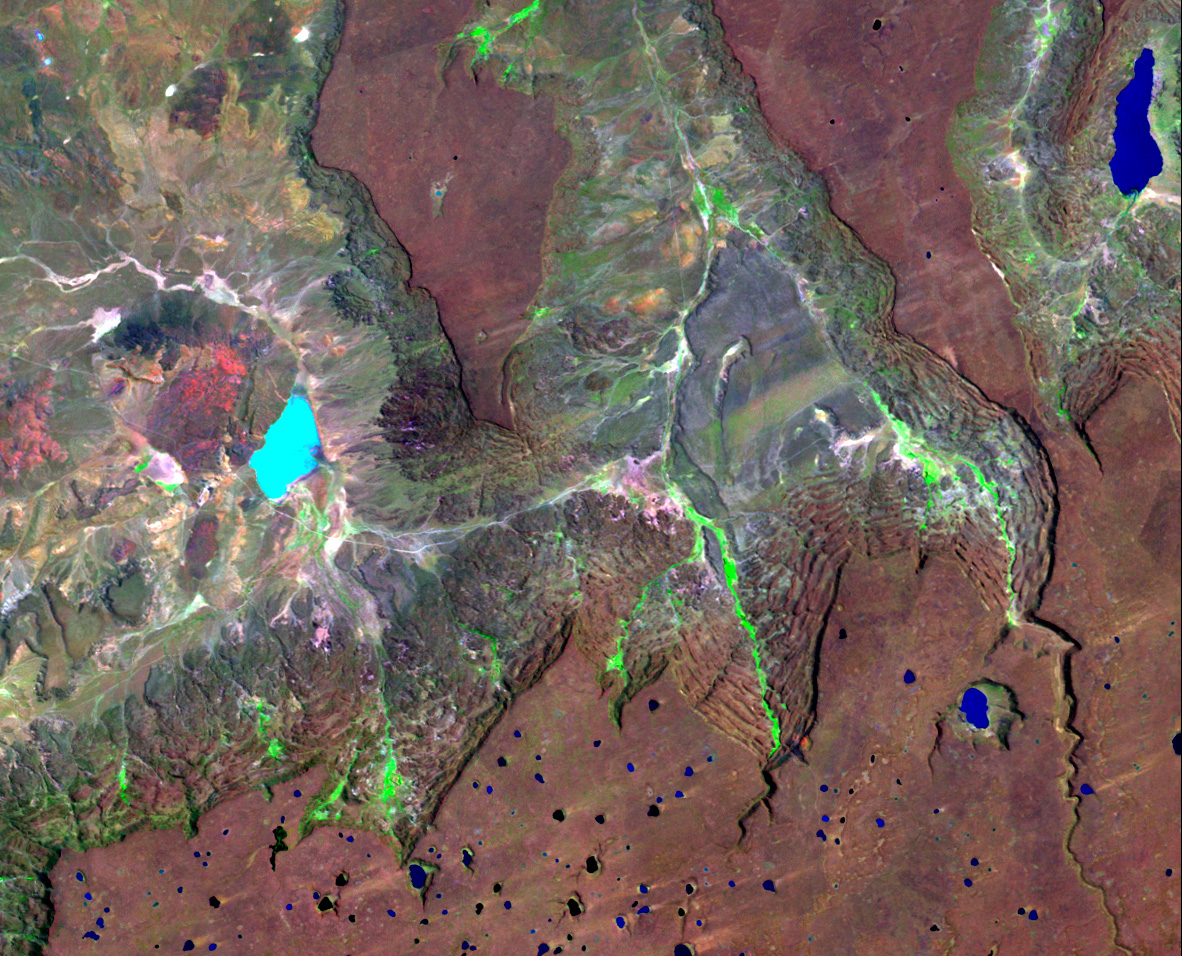
\includegraphics[width=0.4\textwidth]{statement/srtm_l7_basalt.jpg}
    \label{fig:real-view}
  }
 \hspace{0.05\textwidth}
  \subfloat[Image acquired from \ac{SRTM}
  conforming a 3D image.]{
    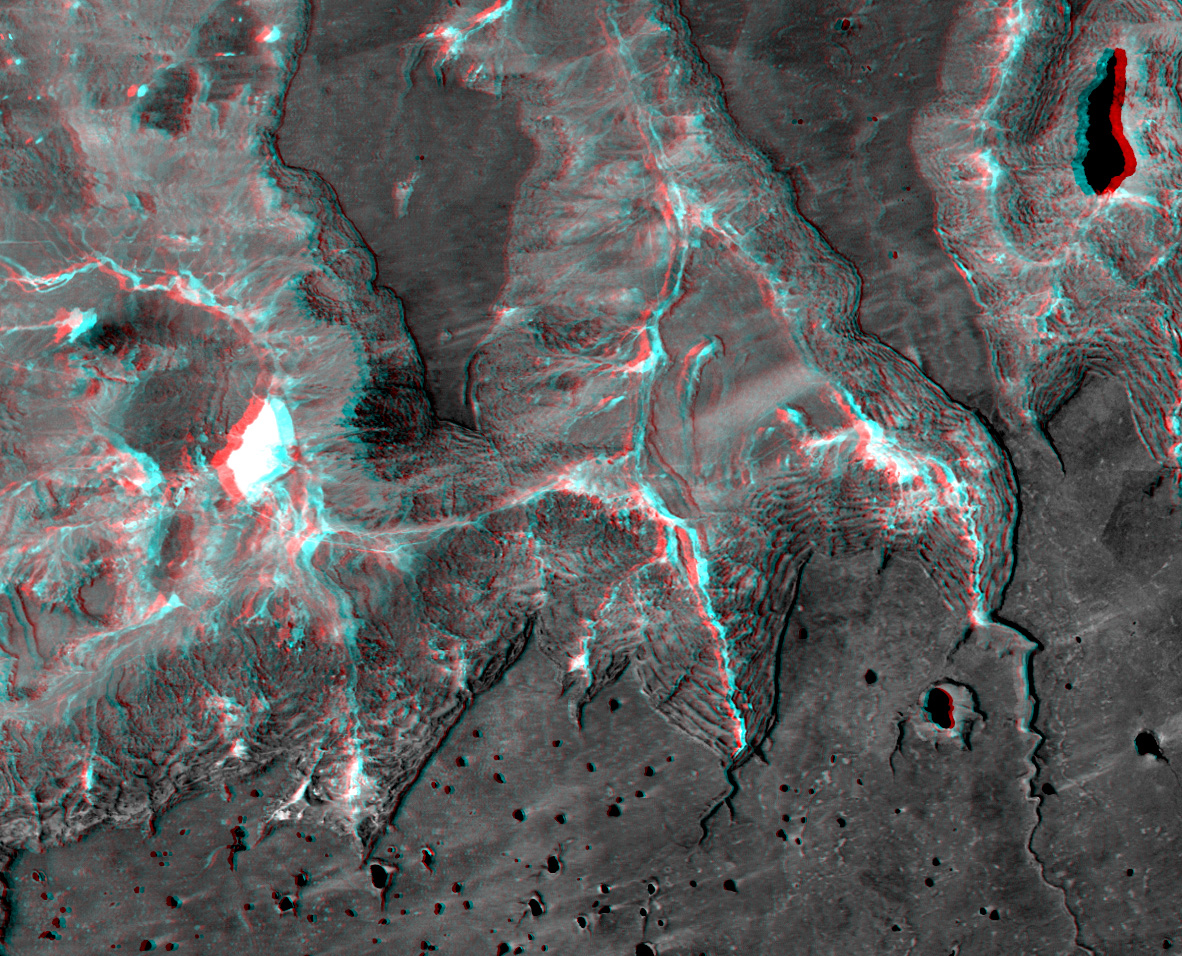
\includegraphics[width=0.4\textwidth]{statement/srtm_anaglyph_basalt.jpg}
    \label{fig:3d-image}
  }
\caption{Different images acquired by \acs{USGS}/\acs{NASA} Landsat.}
\end{center}
\end{figure*}

% \begin{multicols}{2}

% \begin{figure*}
% \begin{center}
% 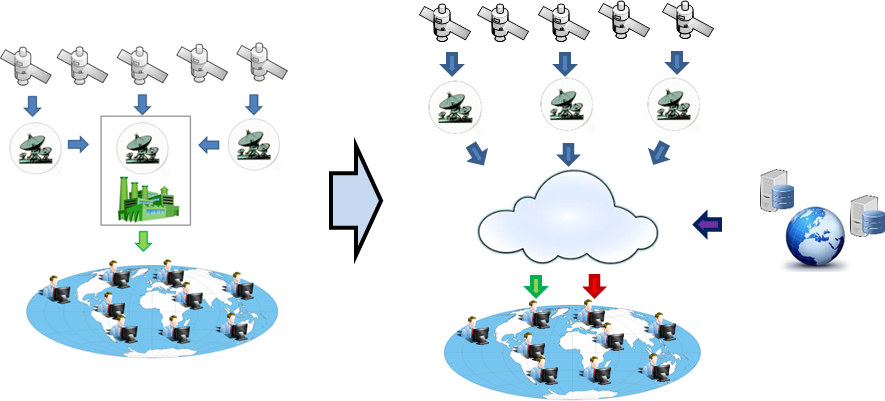
\includegraphics[width=0.2\textwidth]{statement/geocloudConcept.png}
% \caption{The}
% \label{fig:intr-geocloudConcept}
% \end{center}
% \end{figure*}
% \vfill
% \columnbreak
% \begin{figure*}
% \begin{center}
% 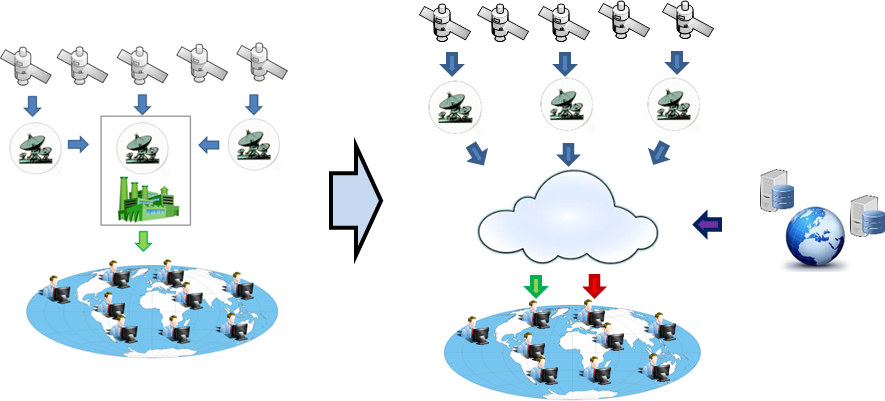
\includegraphics[width=0.2\textwidth]{statement/geocloudConcept.png}
% \caption{The}
% \label{fig:intr-geocloudConcept}
% \end{center}
% \end{figure*}
% \end{multicols}

The geometric resolution is selected depending on how much definition the
telescopes or imaging sensors have. Some examples are the acquisition of a cloud
for weather applications, about $100km$ resolution, or monitoring of roads and
highways for traffic monitoring purpose, under $1m$ resolution.

The temporal resolution is the related to the visit frequency between two
consecutive acquisitions of the same location. This is known in remote sensing
as revisit time. Depending on the
image application, the revisit time can vary. For example, for environmental
monitoring, geology or precision agriculture the revisit time is longer that the
required revisit time for military or maritime surveillance~\cite{Sandau2009}.

\begin{figure}[!h]
\begin{center}
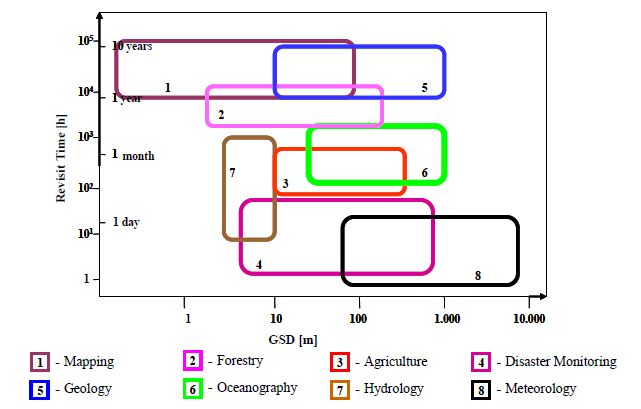
\includegraphics[width=0.9\textwidth]{detaildesign/gsd-revisit-time.png}
\caption{Earth Observation request: GSD vs Revisit Time}
\label{fig:intr-gsd-revisit-time}
\end{center}
\end{figure}



The main component to carry out \ac{EO} imaging consists of the platform.There, the
payloads for image acquisition are installed. These platforms can be summarized
in two groups: spacecrafts and aircrafts. Aircrafts involve aerodines (planes,
and helicopters among others) and aerostats (balloons and
dirigibles). Spacecrafts are systems designed to fly over the atmosphere and
could be used for many different purposes such as communications,remote sensing,
meteorology and planetary exploration among others.


\section{Cloud Computing}

Traditional business applications have always been too expensive and complex. The number and variety of necessary hardware and software to run them
is overwhelming. A team of experts that can install, configure, test, run,
secure, and update is needed in most of cases.
Thanks to Cloud Computing, these
complexities do not exist because it is not necessary to manage the hardware
and software to run the application: it is the responsibility of an experienced cloud provider. The
shared infrastructure makes it work like a utility: You only pay for what you
need, upgrades are automatic and the enlargement or reduction of the service
comprises a simple process.

The NIST~\cite{P.Mell2011} defines \emph{Cloud Computing} as \emph{``Cloud computing is a model for enabling ubiquitous, convenient, on-demand network access to a shared
pool of configurable computing resources (e.g., networks, servers, storage, applications, and services) that
can be rapidly provisioned and released with minimal management effort or
service provider interaction''}.

Several cloud modalities are implemented at present. These are:
\begin{itemize}
\item \emph{Private Cloud:} It is used and operated by a single organization.
\item \emph{Community Cloud:} Organizations that have shared subjects create
  this kind of cloud in which the management and support are carried out by the
  organizations themselves.
\item \emph{Public Cloud:} It is provisioned for  general public used. The
  management of the infrastructure is performed by an academic, companies or
  public organizations.
\item \emph{Hybrid Cloud:} Cloud composed by different infrastructures such as
  public,   community or private in order to achieve some specific objectives.
\item \emph{Federated Cloud:} Nowadays, this kind of infrastructures have
  increasing interest. The federated architectures are a combination of community, public
  and hybrid clouds in which each of them offer features that the consumer can
  use in a transparent manner, i.e. the user can use the whole infrastructures
  as if it was a single entity that internally manages all the processes and
  infrastructures that constitute it. In the section~\ref{subsec:federatedtools} are detailed.
\end{itemize}

The  cloud computing features are summarized as follows:
\begin{itemize}
\item \emph{On-demand self-service:} A cloud computing user can provision,
  deploy and release computing resources as needed automatically without human
  interaction.
\item \emph{Broad network access:} Cloud capabilities can be accessed by
  standard mechanisms or client platforms.
\item \emph{Resource pooling:} Different resources can be assigned such as memory,
  processing capability and network bandwidth among others.These can be
  geographically distributed or into several cloud machines.
\item \emph{Rapid elasticity:} Resources can be elastically provisioned and
  automatically released. This features facilitates fast scalability of resources.
\item \emph{Measured Service:} Resources can be monitored, controlled and
  reported in order to achieve transparency for the cloud supporter and consumer.
\end{itemize}

The cloud computing infrastructure offers different kinds of services that are
summarized as follows:

\begin{itemize}
\item \emph{\ac{SaaS}:} It is the capacity provided to the consumer
  to use  the infrastructure with provider's applications.
\item \emph{\ac{PaaS}:} It is the capacity provided to the consumer which 
  consists of the  applications created by the consumer using languages, libraries
  and tools supported by the platform owner, can be deployed on the cloud.
\item \emph{\ac{IaaS}:} The capacity provided to the
  consumer consists of provisioning computing resources in order to facilitate
  the deployment and run its developed software.
\end{itemize}



\section{The Fed4FIRE European Project}%
The \emph{Fed4FIRE}~\cite{Fed4FIRE2014a} is an Integrating Project under the European Union's
\ac{FP7} in the topic \emph{Future
  Internet Research and Experimentation}. The project is performed by a
consortium of 29 partner from different countries. The project is coordinated by
 \emph{iMinds}, Belgium.
The \emph{Fed4FIRE} project establishes a common federation framework for
experimenters. A large  number of European facilities are integrated. Such facilities focus on different  areas
of networking. Some example domains are wireless networking, cloud computing, smart
cities and grid computing among others.
Furthermore, one of the main objectives of the \emph{Fed4FIRE} project is the
validation of its infrastructure to perform
innovative experiments. Then, one of the objectives of the GEO-Cloud experiment
is to test and validate the \emph{Fed4FIRE} infrastructure to carry out large
scale, industry driven innovative experiments.

\section{The Geo-Cloud Experiment Overview}


\subsection{Experiment Description}

The experiment consists of virtualizing a conventional Earth Observation system to offer on
demand services with the objective of validating its viability, find
the strengths and weaknesses of using cloud computing technology and establish
possible solutions for a future implementation in the market. There are three
components:
\begin{enumerate}
\item \emph{In-orbit mission:} this component generates the raw data. This
  consists of un-processed images of the Earth captured by a constellation of
  satellites and downloaded to a distributed network of ground stations.
\item \emph{Data Centre computed in cloud:} the data has to be stored, processed at different levels based on the services offered and distributed to the clients. The data acquired by the in-orbit mission is integrated with other sources to provide higher quality services.
\item \emph{End-users:} users of the provided services with different levels of remote access rights.

\end{enumerate}


\subsubsection{Experiment Design}


The GEO-Cloud experiment requires emulating a complete realistic Earth Observation mission to provide high added value services such as crisis management. To this complex situation, the system has to response by processing on demand massive and variable amounts of stored and on line transferred data.

GEO-Cloud makes use of the following \emph{Fed4FIRE} facilities: \pl,\vw and
\bonfire. \pl allows us to measure real network characteristics, geographically
distributed, to setup our models. \vw allows us to create any desired network
topology and emulate the in-orbit mission and the web service to the
users. \bonfire provides us a real cloud infrastructure with observability in
all the layers to test our cloud based services.


\paragraph{Implementation of the acquisition of geo-data in Virtual Wall and
  PlanetLab}~\\
The acquisition of geo-data is obtained from the in-orbit mission. The
constellation of satellites and the ground stations are emulated in \vw. A
network topology is implemented to communicate the different satellites with the
ground stations. Every satellite in its orbit and every ground station models
are simulated in a different node.

The satellite models simulate the orbits and the pass of the satellites over the
ground stations. The ground stations models simulate the coverage of the
antennas and the download of the data. When a satellite is inside this radius,
the satellite downloads the data to the ground station. Then, the downloaded data in the ground stations is transferred to the \bonfire cloud.

With the \vw network,the \emph{bandwidths, latencies and loss rates} are
controlled.Also a realistic network topology to transfer data between different
nodes is created.

In order to determine the correct link characteristics for the connections
between the ground and the cloud infrastructure, a profiling tool has been
developed for measuring appropriate values for the link impairment between these different geographical locations using the \pl testbed.


\paragraph{Implementation of the cloud based services in BonFIRE}~\\
To facilitate offering the previous services we propose to implement a multi-layered cloud model in the \bonfire cloud infrastructure to generate on demand geo-information. The multi-layered cloud model is constituted of two layers:
\begin{itemize}
\item \emph{Layer 1:} This layer involves the basic satellite imagery services.  It acquires the raw data, stores it, has the first level of processing, distributes the processed data and offers the hosting service.

\item \emph{Layer 2:} This layer involves the high added value services. It can use historical processed, real time captured and pre-processed data from Layer 1. This layer processes the information for real time generation of geo-information and offers real time access and distribution to the end-users. Typically, the implementation of high added value EO services involves the ingestion of the raster imagery from the satellites into a spatial database or storage, where it can be refined, simplified, processed or combined with other data sources in vector or raster format. The products, which can be vector or raster data, are distributed or queried using Internet technologies (\ac{OGC} standards like \ac{WMS}) or through Web services (tiles, caches, etcetera).
\end{itemize}

Thus, the whole \ac{EO} system is completely implemented in \emph{Fed4FIRE} (see Figure 3).

\begin{figure}[!h]
\begin{center}
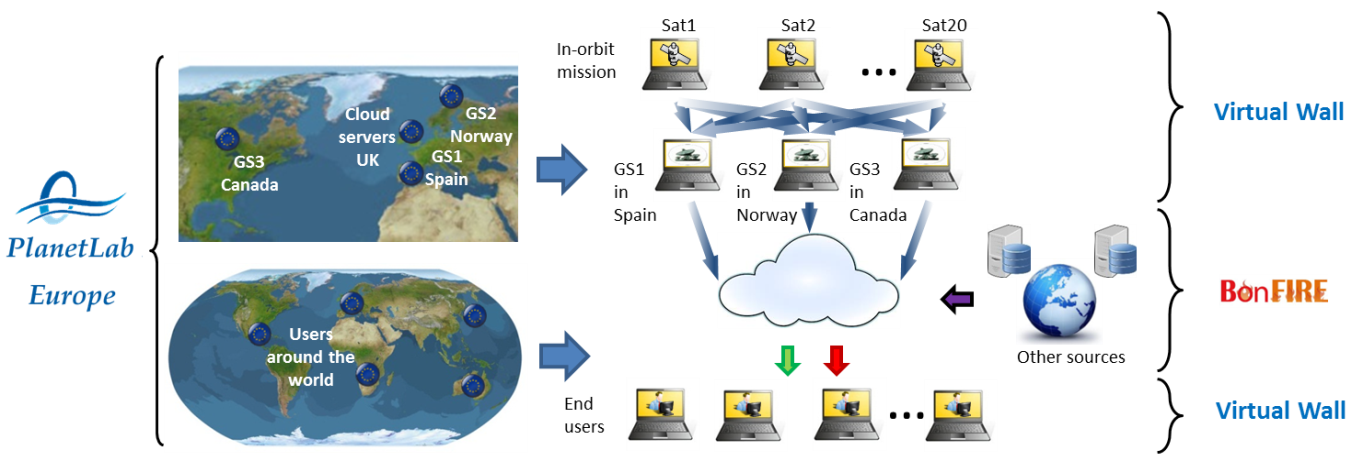
\includegraphics[width=1.1\textwidth]{statement/testbeds-geocloud.png}
\caption{Geo-Cloud implementation in Fed4FIRE}
\label{fig:intr-testbeds-geocloud}
\end{center}
\end{figure}




\subsection{Impact in Fed4FIRE}
The experiment will contribute to several objectives of the \emph{Fed4FIRE}
project:
\begin{itemize}
\item GEO-Cloud will increase trustworthiness of its facilities and support their
sustainability. 
\item GEO-Cloud will test \emph{Fed4FIRE} tools for its use in the industry
driven experiments close to market, specifically complex and real time services
for Earth Observation industry when critical situations occur.
\item GEO-Cloud will validate the tools for monitoring and control of cloud computing
and networking in EO services for emergencies and will test the limits of the
infrastructure for processing, storing and traffic of massive on-demand
data. 
\item GEO-Cloud will provide feedback to improve the infrastructure during and
after the experiment is carried out, sharing our knowledge in traditional
infrastructures for \ac{EO} applications, monitoring, processing and
distribution of geospatial data.
\end{itemize}

\subsection{Scientific and Technological Impact}

GEO-Cloud will contribute to the development of a common framework to provide worldwide services in the Earth
Observation field. It will answer if Future Internet technologies can provide
viable solutions for the complex \ac{EO} market and will find the limitations of
the current cloud computing technology for its application in Earth Observation.

\subsection{Socio-Economic Impact}

The Geo-Cloud project is used as a framework to offer services from \ac{EO}
users. The benchmark developed in the experiment allows us to establish the
frontiers of viable and not viable cloud solutions in \ac{EO} depending on the
type of demand and service offered. This will establish the basis to satisfy the
growing demand of added value \ac{EO} services.

The reduction of the processing, storage, communications and distribution costs
of \ac{EO} services will facilitate the access to the remote sensing technology to
common end users, but also to a more general public. GEO-Cloud will contribute
in the definitio of the basis to advance in the use of geospatial information of the nine
``Societal Benefit Areas'' defined in GEO: disasters, health, energy, climate,
water, weather, ecosystems, agriculture and biodiversity; by demonstrating
whether or not cloud computing offers technologically and economically viable
solutions to offer highly demanding services.

The results obtained in the experiment will be used by \emph{Elecnor Deimos} to offer new
services to the general public, current end users and future potential users. The users will be beneficiated since we will define the framework to
offer higher quality services.




\section{Document Structure}

This document has been carried out as Master Thesis rules from the \emph{Escuela
Superior de Informática} of the \emph{Universidad de Castilla-La Mancha}. It contains
the following sections:


\begin{definitionlist}
\item[Chapter \ref{chap:antecedentes}: \nameref{chap:antecedentes}] In this
  chapter an overview of the necessary knowledge areas is made to study for the
  development of GEO-Cloud, like cloud computing, distributed middleware,
  processing premises for \ac{EO} and several testbeds in \emph{Fed4FIRE}.
\item[Chapter \ref{chap:objetivos}: \nameref{chap:objetivos}] In this
  chapter, the main objectives for GEO-Cloud are depicted and explained.
\item[Chapter \ref{chap:method}: \nameref{chap:method}] in this chapter the
  selected methodology is explained and justified. Also, the uses resources such
  \emph{Fed4FIRE's} testbeds, hardware and software are depicted.
\item[Chapter \ref{chap:geocloud-experiment}: \nameref{chap:geocloud-experiment}] In this
  chapter, the entire GEO-Cloud project is explained. The design and implementation of the
  satellite constellation, the design and implementation of the satellites and
  ground stations simulators over \vw, the design and implementation of the
  cloud architecture for \ac{EO} and finally the \pl experiment for acquiring
  network impairments are detailed.
\item[Chapter \ref{chap:evolution}: \nameref{chap:evolution}] In this chapter,
  the project evolution during the development detailing the phases and
  iterations besides the inconveniences and decisions to solve them are
  described. Also, costs of project and schedule are shown.
\item[Chapter \ref{chap:results}: \nameref{chap:results}] In this chapter, the
  results of the development of the project are shown.
\item[Chapter \ref{chap:conclusions}: \nameref{chap:conclusions}]In this
  chapter, the development conclusion and the reached objectives are
  summarized. Some future work and lines of research are suggested.
 \end{definitionlist}
